%BEGIN LATEX
\typeout{}
\typeout{\space\space\space\space\space
         The title page being created is a LaTeX approximation of a fancy}
\typeout{\space\space\space\space\space
         PostScript cover page.  All the fancy cover pages for the HOL}
\typeout{\space\space\space\space\space
         Manual may be generated if you have (1) a PostScript printer,}
\typeout{\space\space\space\space\space
         (2) the "psfig" TeX macros, and (3) a DVI to PostScript converter}
\typeout{\space\space\space\space\space
         that understands these macros.  The cover pages may be found in}
\typeout{\space\space\space\space\space
         ../LaTeX/Covers, and shoud be made pursuant to the instructions}
\typeout{\space\space\space\space\space
         given in ../LaTeX/Covers/READ-ME.}
\typeout{}




\begin{titlepage}
\null\vskip-47pt
\hbox to \textwidth
{\bf [For \holn{} \holnversion] { \hfil \today}}

\setcounter{page}{1}                      % titlepage IS page 1

\vspace*{60mm}


\begin{center}
 {\Huge\bf The HOL System}\\[0.4cm]
{\LARGE\bf TUTORIAL}\\[2.5cm]
\end{center}

\begin{center}
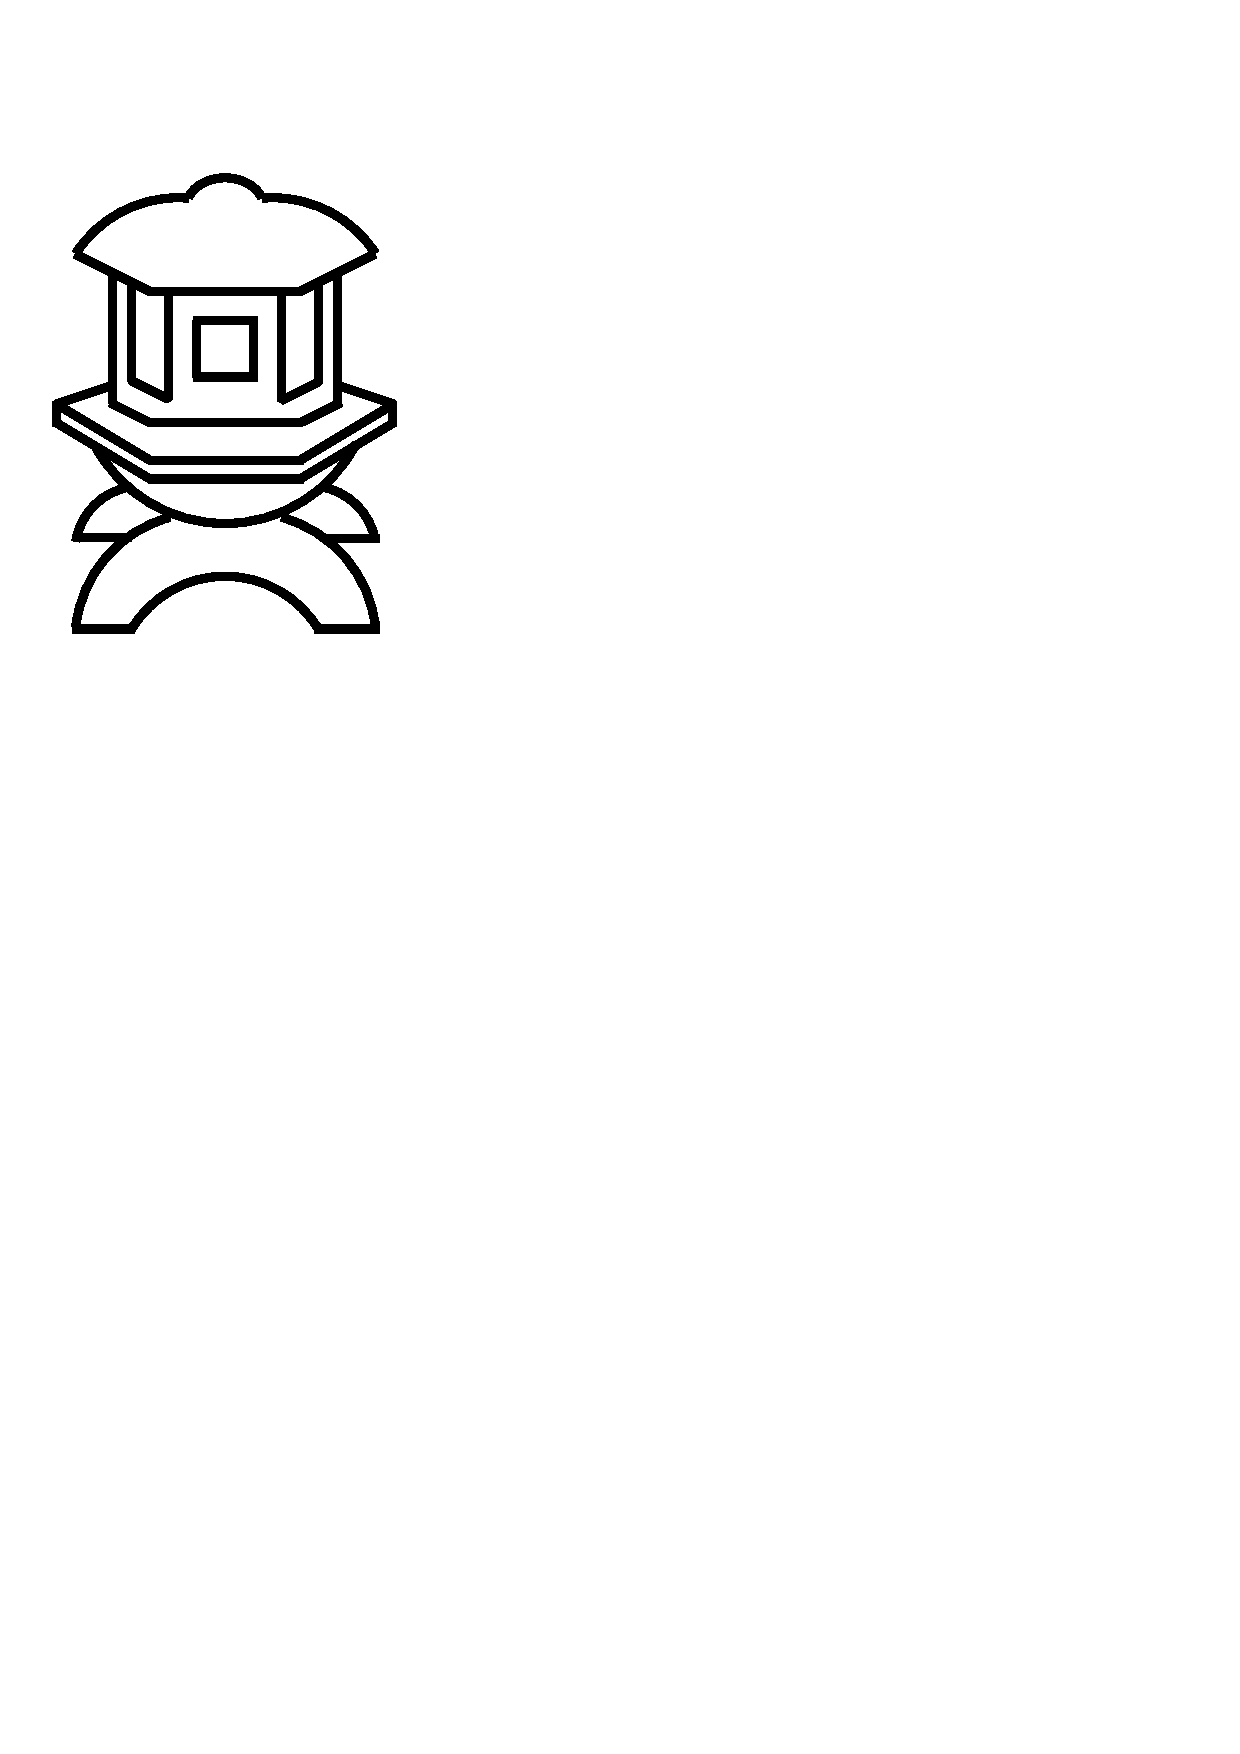
\includegraphics[width=3cm]{../Logo/logo}
\end{center}


\vfill
\end{titlepage}

% To kick a blank page with no header
\thispagestyle{empty}
\mbox{}
\newpage
%END LATEX

%HEVEA \begin{tabular}{l@{\hspace{5cm}}r}
%HEVEA {\bf [For \holn{} \holnversion]} & \today\\
%HEVEA \end{tabular}
%HEVEA
%HEVEA \begin{center}
%HEVEA {\Huge\bf The HOL System}\\
%HEVEA {\LARGE \bf TUTORIAL}\\
%HEVEA \vspace{1cm}
%HEVEA \begin{toimage}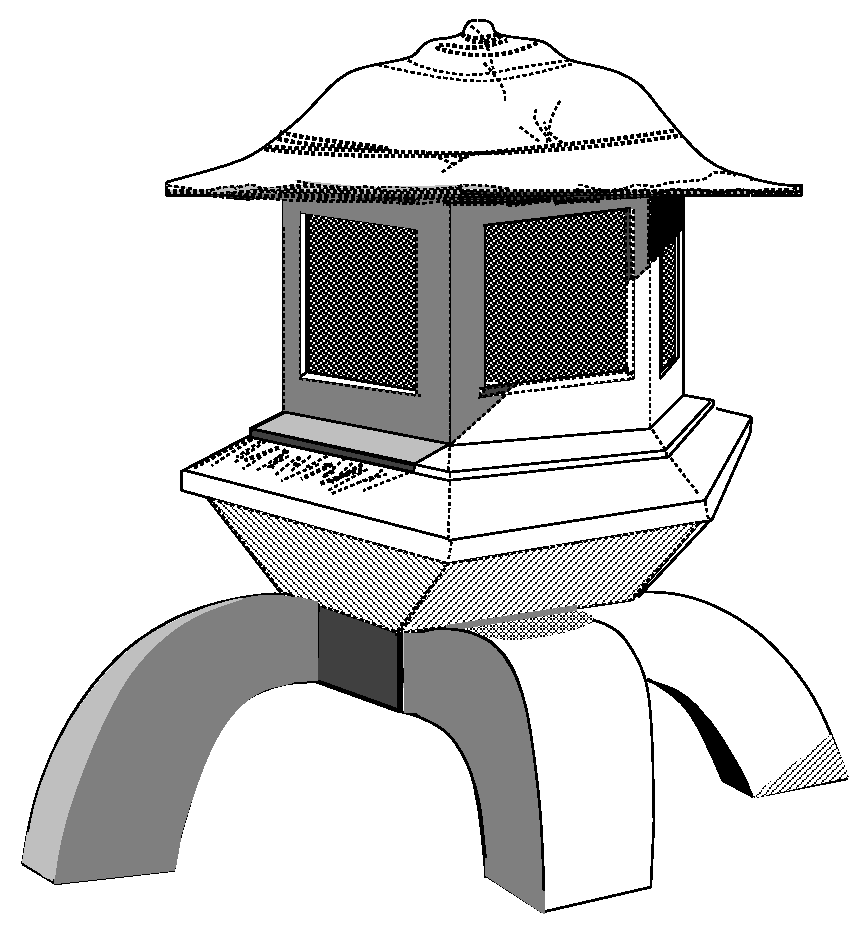
\epsfig{file=../Covers/LANTERN.ps,height=2.5in}\\
%HEVEA \end{toimage}\imageflush
%HEVEA \begin{tabular}{ccc}
%HEVEA University of Cambridge & \hspace*{10ex}DSTO\hspace*{10ex} & SRI International
%HEVEA \end{tabular}
%HEVEA \end{center}




%%% Local Variables:
%%% mode: latex
%%% TeX-master: "tutorial"
%%% End:
